\documentclass[aip,jcp,reprint,a4paper,onecolumn,nofootinbib,amsmath,amssymb]{revtex4-1}
% Options for onecolumn and a4paper
\linespread{1.0}
\usepackage[expansion,protrusion,tracking=smallcaps]{microtype}
\usepackage{chemformula,tikz}
\usepackage{listings,xcolor}
\lstset{
  basicstyle = \small\ttfamily,
  keywordstyle = \color{blue!80!black},
  commentstyle = \color{green!40!black},
  columns = fullflexible,
  xleftmargin = 1em
}
\lstdefinelanguage{espresso}[]{TCL}{%
  morekeywords={setmd,thermostat,constraint,inter,part,integrate,lbfluid,lbboundary,writevtk,reaction},
  deletekeywords={range}
}
\lstnewenvironment{espresso}[1][]%
  {\lstset{language=espresso,#1}}%
  {}
\lstnewenvironment{bash}[1][]%
  {\lstset{keywordstyle = \color{red!80!blue},keywords={\$},#1}}%
  {}
\usepackage{xspace}
\newcommand\code{\lstinline}
\newcommand{\es}{\mbox{\textsf{ESPResSo}}\xspace}
\newcommand\codees{\lstinline[language=espresso]}
\begin{document}
\title{Catalytic Reactions Tutorial}
\author{Joost de Graaf}
\email[]{\texttt{jgraaf@icp.uni-stuttgart.de}}
\affiliation{Institute for Computational Physics,
  Universit\"at Stuttgart,
  Allmandring 3,
  D-70569 Stuttgart,
  Germany}
\affiliation{School of Physics and Astronomy,
  University of Edinburgh,
  Scotland, Edinburgh EH9 3JL,
  United Kingdom}
\author{Henri Menke}
\email[]{\texttt{henri@icp.uni-stuttgart.de}}
\affiliation{Institute for Computational Physics,
  Universit\"at Stuttgart,
  Allmandring 3,
  D-70569 Stuttgart,
  Germany}
\date{\today}

\begin{abstract}
  Catalytic reactions
\end{abstract}

\maketitle

\section{Cataltic Reactions}

There are processes in nature which do not occur at reasonable
temperatures because the energy penalty is too high to be overcome by
mere fluctuations.  The activation energy of such processes can in
some cases be lowered significantly in the presence of a catalyzer.

We may write a general reaction as
\begin{equation}
  \label{eq:equi}
  \ch{!(reactants)(R) <=> !(products)(P)}
\end{equation}
where \ch{R} are the reactants and \ch{P} are the products.  The
double headed arrow suggests that this reaction is in a equilibrium,
i.e.~the rate of the forward reaction is the same as the rate of the
back reaction and can also be zero.  A catalyzer shifts the free
energy landscape in favour of one of the constituents \ch{R} and
\ch{P}.  We choose \ch{P}, since it stands for the products and we
want to enhance the forward reaction.
\begin{equation}
  \ch{!(reactants)(R) <=>>[ !(catalyzers)(C) ] !(products)(P)} \;.
\end{equation}
If the back reaction rate is tiny it eventually becomes negligible and
the reaction only occurs in one direction.
\begin{equation}
  \label{eq:cat}
  \ch{!(reactants)(R) ->[ !(catalyzers)(C) ] !(products)(P)} \;.
\end{equation}

The equilibrium reation~\eqref{eq:equi} can be described by the
equilbrium reaction constant
\begin{equation}
  \label{eq:const}
  K_{\text{eq}} = \frac{k_{\text{eq},+}}{k_{\text{eq},-}} = \frac{[\ch{P}]}{[\ch{R}]}
\end{equation}
with $[\ch{P}]$ and $[\ch{R}]$ the product and reactant concentration
and $k_{\textrm{eq},\pm}$ the forward and backward reaction rates.
The chief effect of the reaction is a change of the concentrations of
reactants and products over time.  We find the following coupled
differential equations
\begin{subequations}
  \label{eq:diff}
  \begin{align}
    \label{eq:diff-equi-a}
    \frac{d[\ch{R}]}{dt} &= + k_{\text{eq},-}[\ch{P}] - k_{\text{eq},+}[\ch{R}] \;, \\
    \label{eq:diff-equi-b}
    \frac{d[\ch{P}]}{dt} &= - k_{\text{eq},-}[\ch{P}] + k_{\text{eq},+}[\ch{R}]  \;.
  \end{align}
  In the case of excessive catalysis~\eqref{eq:cat} the back reaction
  rate $k_{\text{eq},-}$ can be set to zero and the forward reaction
  rate is enhanced $k_{\text{eq},+} \to k_{\text{ct}}$.  The rate
  equations then coalesce to
  \begin{equation}
    \label{eq:diff-cat}
    -\frac{d[\ch{R}]}{dt} = \frac{d[\ch{P}]}{dt} = k_{\text{ct}}[\ch{R}] \;.
  \end{equation}
\end{subequations}

The reaction move is a stochastic process and takes place with a
certain probability, depending on the reaction rate
\begin{equation}
  \label{eq:prob}
  P_{\text{move}} = 1 - \mathrm{e}^{-k\,\Delta t}
\end{equation}
with the reaction rate $k \in \{ k_{\text{eq},+}, k_{\text{eq},-},
k_{\text{ct}} \}$ and the simulation time step $\Delta t$.

\section{Cataltic Reactions in \es}

There are two implementations of the reaction
scheme~\eqref{eq:diff-equi-a},~\eqref{eq:diff-equi-b},
and~\eqref{eq:diff-cat}, which we will refer to as \emph{number
  conserving} and \emph{not number conserving}.  In the following we
will find out what this actually means.

\subsection{Not Number Conserving Scheme}

In \es\ we assume the equilibrium constants in
equations~\eqref{eq:diff} to be equal, i.e.~$k_{\text{eq},+} =
k_{\text{eq},-}$.  Thus, according to~\eqref{eq:const}, the reaction
constant $K = 1$.  The equilibrium constant is applied to all the
particles in the system and determines the conversion rate between the
reactants and products.  For reactants in the vicinity of the
catalyzer the forward reaction is favoured and no back conversion will
take place there.  Also the forward reaction rate is enhanced to
$k_{\text{ct}}$ and can be specified as an input parameter.

\begin{figure}
  \centering
  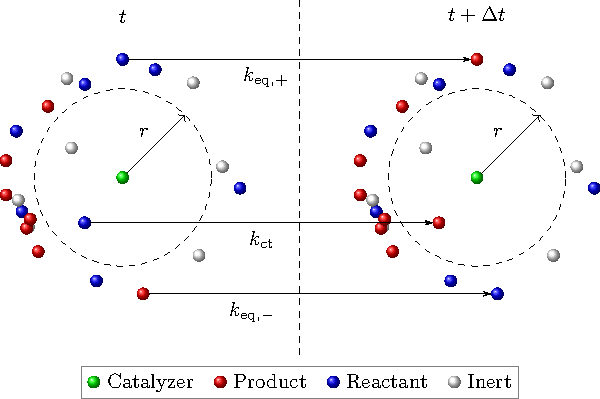
\includegraphics{FIGURES/non-number-conserving}
  \caption{Illustration of the \emph{not number conserving} scheme.
    One the left and on the right hand side the same simulation is
    depicted at time steps $t$ and $t+\Delta t$, respectively.  The
    active reaction leads to a conversion of three particles in this
    example, two of these in the bulk and one within the reaction
    range of the catalyzer.  Even though $k_{\text{eq},+} =
    k_{\text{eq},-} = k_{\text{eq}}$ in \es, we show them seperately
    to emphasise that one is a forward and one is a back reaction.}
  \label{fig:nnc}
\end{figure}

FIG.~\ref{fig:nnc} shows the reaction scheme explained before
pictorially.  Within one time step bulk reactions take place with the
equilibrium constant.  These might occur in both directions.  Within
the reaction range, determined by $r$, the equilibrium reactions are
also allowed to take place, but additionally the forward reaction is
catalysed.  From this we already see, that it does not make sense to
set $k_{\text{eq}} > k_{\text{ct}}$.  This would basically shadow the
effect of the catalyzer in contrast to the equilibrium reactions in
bulk.

By looking at the sketch in FIG.~\ref{fig:nnc} and carefully following
the discussion of the scheme above, we may now have understood why the
scheme is called \emph{not number conserving}.  The problem is, that
forward and backward reaction are not balanced.  Even though the
overall number of particles is conserved the number of particles per
species is not.  This is evident from the sketch, where we have two
reactants and one product before the reaction and one reactant and two
products after the reaction.  This issue can be rectified in the
\emph{number conserving} scheme.

\subsection{Number Conserving Scheme}

The fix to the issue of lacking number conservation discussed above is
simple.  We disallow bulk reactions of single particles\footnote{We
  noticed that we set the equilibrium reaction rate $k_{\text{eq}} =
  0$ in most cases anyway.} and allow a reaction inside the reaction
range only in rectant-product pairs.  Simply exchanging the particles
in the pair would not yield a large effect, which is why we introduce
an additional notion of symmetry breaking.  Consider a Janus particles
which is coated with \ch{Pt} on one hemisphere and with \ch{Au} on the
other hemisphere.  Both surfaces enhance a reaction,
here\cite{Gibbs_10,Wheat_10}
\begin{align}
  \label{eq:H2O2}
  \ch{
    H2O2 &->[ Pt ] 2 H^+ + 2 e^- + O2 \\
    2 H^+ + 2 e^- + H2O2 &->[ Au ] 2 H2O
  }
\end{align}
This reaction is depicted in FIG.~\ref{fig:janus}.  The large arrow in
the sketch points in the direction of movement induced by the
reaction.  We refer to upper and lower hemisphere or half-space in the
following, where upper and lower are to be seen in the direction of
propulsion.  In the present case \ch{Au} is the upper hemisphere and
\ch{Pt} is the lower hemisphere.

\begin{figure}
  \centering
  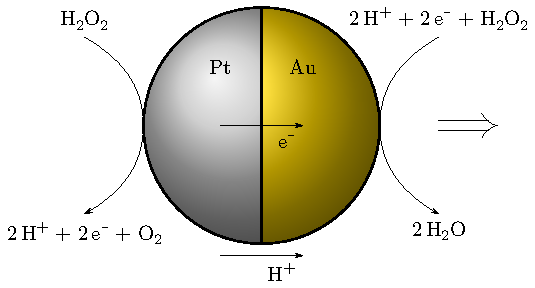
\includegraphics{FIGURES/janus-particle}
  \caption{A Janus particle, coated with a catalytic surface on both
    hemispheres may support two different reactions.  This results in
    breaking of rotational and reflection symmetry which propells the
    particle in the direction of the large arrow.}
  \label{fig:janus}
\end{figure}

For simplicity in the simulation we abstract away all the reaction
mechanism including the electron transport through the Janus particle
and the proton transport around it.  We end up with a simple scheme,
depicted in FIG.~\ref{fig:nc}.

As already explained, reactions can only take place for
reactant-product pairs.  The conversion is such that a reactant is
converted to a product and a product is converted to a reactant.  This
obviously ensures conservation of the particle number of each type,
respectively.  To model a Janus particle as in FIG.~\ref{fig:janus} we
allow the exchange move to only take place for a chosen configuration.
For the pair to be eligible for the reaction move, the following
conditions have to be met:
\begin{enumerate}
\item Both partners of the reactant-product pair have to reside within
  the reaction range.
\item The product has to reside in the upper half-space of the
  reaction range..
\item The reactant has to reside in the lower half-space of the
  reaction range.
\end{enumerate}
This is again described pictorially in FIG.~\ref{fig:nc}.

\begin{figure}
  \centering
  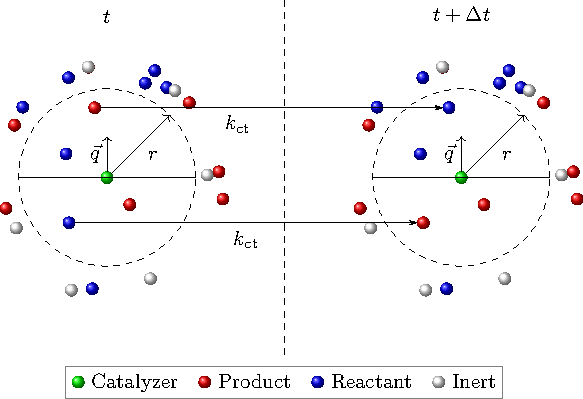
\includegraphics{FIGURES/number-conserving}
  \caption{Illustration of the \emph{number conserving} scheme.  One
    the left and on the right hand side the same simulation is
    depicted at time steps $t$ and $t+\Delta t$, respectively.  The
    active reaction leads to a conversion of one reactant-product pair
    of particles in this example.  We can see, that only a well
    positioned pair is converted.  The second reactant-product pair
    within the reaction range is not viable for conversion.}
  \label{fig:nc}
\end{figure}

\subsection{Usage in \es}

Capabilitiy for catalytic reactions can be enabled in \es\ by
compiling with the equally named feature \code{CATALYTIC_REACTIONS}.
The number conserving method additionally requires the \code{ROTATION}
feature to give the particles an orientation vector.  In \es{} the
orientation of the particle is defined by a quaternion; this in turn
defines a rotation matrix that acts on the particle's initial
orientation (along the z-axis), which then defines the particles
current orientation~\cite{UG,Limbach_06,Arnold_13}.

In \es\ particles are set up using the \codees{part} command.  It
allows to set various options, such as the initial position
(mandatory), the type or the charge.  To setup the reaction there is
the \es\ command \codees{reaction}, which operates on particle types.
The general syntax is
\begin{espresso}
reaction reactant_type R catalyzer_type C product_type P range r ct_rate k_ct
    [eq_rate k_eq] [react_once on/off] [swap on/off]
\end{espresso}
The parameters in square brackets are optional and can be left out.
They will then assume their default values which are \codees{eq_rate 0.0},
\codees{react_once off}, and \codees{swap off}.

\noindent\textbf{Important:} Due to the method of implementation there
can only be one reaction.  You can alter the reaction parameters, but
you may not change the reaction partners.

To set up a reaction between the types 1 and 2, where particles of
type 3 act as catalyzers with a reaction range of 1.5 around them with
a reaction rate of 20, one types
\begin{espresso}
reaction reactant_type 1 catalyzer_type 3 product_type 2 range 1.5 ct_rate 20
\end{espresso}
Here we have left out the optional parameters, but their meaning is
nevertheless important.  The first one, \codees{eq_rate}, should be
self explanatory; it sets the equilibrium reaction rate as detailed in
the introductory sections.  The \codees{react_once} parameter
determines whether a particle can take part in a only single reaction
move per time step.  In the case of multiple catalyzers in the system
a particle might be tagged for reaction several times by different
catalyzers because their reaction ranges overlap and the reactant is
inside this overlap.  This can be prevented by setting
\code{react_once on}.  That way the reaction rate is independent of
the density of catalyzers.  Finally, the parameter \codees{swap}
determines which scheme to use; \codees{swap off} uses the not number
conserving scheme, \codees{swap on} uses the number conserving scheme.
The name `swap' originates from the sketch FIG.~\ref{fig:nc}, because
it looks as if the particles are swapped.

However, the \codees{swap} option does not really swap the particles,
but only exchanges their type (and their charge, if \es\ was compiled
with \code{ELECTROSTATICS}).

\section{Configuring \es\ for Catalytic Reactions}

For this tutorial to work you need a version of \es\ containing the
catalytic reactions feature with the \codees{swap} mechanism.
Therefore check out the \es\ online repository at
\url{https://github.com/espressomd/espresso}.  If you have installed
\code{git}, you can issue on the command line
\begin{bash}
$ git clone https://github.com/espressomd/espresso.git
\end{bash}
Now you are ready to build \es.  Change to the newly created directory
and use the following commands to configure \es\ for compilation.
\begin{bash}
$ mkdir build
$ cd build
$ cmake ..
\end{bash}
After this, you will need to copy the \code{myconfig-sample.hpp} file
into \code{myconfig.hpp} and select the appropriate \code{FEATURES} in
the latter.
\begin{bash}
$ cp myconfig-sample.hpp myconfig.hpp
\end{bash}
To run all the tutorials you need to uncomment the following \code{FEATURES}:
\begin{bash}
#define ELECTROSTATICS
#define ROTATION
#define MASS
#define CATALYTIC_REACTIONS
#define LB_GPU
#define LENNARD_JONES
#define VIRTUAL_SITES_RELATIVE
\end{bash}
Now you are ready to build \es{}.
\begin{bash}
$ make -j
\end{bash}
Next you can unpack the archive with the tutorial files in this
directory. You will find two folders, one called `EXERCISES' and one
called `SOLUTIONS'.


\section{Concluding Remarks}

With that, you have come to the end of this tutorial. We hope you
found it informative and that you have a sufficient understanding of
the way to deal with catalytic reactions in \es{} to set up
simulations on your own.

\section*{References}

\bibliographystyle{unsrt}
\bibliography{refs}

\end{document}

%%% Local Variables: 
%%% mode: latex
%%% End:
